\chapter{Cubed-sphere finite-volume methods}
\label{chp-cs-fv}
In this chapter, we demonstrate the application of the dimension splitting method,
presented in Chapter \ref{chp-2d-fv}, to solve the advection equation on the cubed-sphere based on \citet{putman:2007}.
One significant difference is that on the cubed-sphere, special attention must be given to the stencils near the cube edges.
Additionally, when employing ghost cell layers, the flux at the cube edges is computed twice,
requiring treatment to ensure a unique value in order to achieve mass conservation.

This chapter is organized as follows: Section \ref{chp-cs-adv} introduces the advection equation on the cubed-sphere.
Section \ref{chp-cs-fvcs} presents its finite-volume discretization with a focus on the extension of dimension splitting (Section \ref{sec-csdsplit}) 
as presented in Section \ref{sec-dsplit}.
Numerical experiments are presented in Section \ref{chp-cs-numexpadv}, where we use dimension splitting to assess its
accuracy in computing the divergence of a given vector field to check its numerical consistency, as well as to solve the advection equation.
In particular, we explore different treatments for the cube edges. Section \ref{chp-cs-conc} presents the final thoughts.

\section{Cubed-sphere advection equation its integral form}
\label{chp-cs-adv}
Given a tangent velocity field $\boldsymbol{u}$ on the sphere, we denote its
contravariant components by ${u}$ and ${v}$.
We shall use all the notations introduced in Section \ref{cs-notation}.
The advection equation on panel the $p$ of the cubed-sphere with initial condition $q_0$ is given by:
\begin{equation}
	\begin{cases}
	\label{eq1-adv-cs}
	\bigg[{\partial}_t{q}+
	\frac{1}{\sigma}\bigg(
	{\partial}_x{({u} q \sigma)}+
	{\partial}_y{({v} q \sigma)}
	\bigg)\bigg](x,y,p,t)
	= 0,\\
	q(x,y,p,0) = q_0(x,y,p),
	\end{cases}
\end{equation}
$\forall (x,y) \in [-a,a]^2$, $t\in[0,T]$.
We denote by $\nabla \cdot (q\boldsymbol{u})$ the divergence operator:
\begin{equation}
	\label{advcs:eqdiv}
	\nabla \cdot (q\boldsymbol{u})(x, y, p, t) =  \frac{1}{\sigma}
	[{\partial_x (uq\sigma)} + {\partial_y (vq\sigma)}](x, y, p, t).
\end{equation}
We recall that we say the $\boldsymbol{u}$ is \textbf{non-divergent} if $\nabla \cdot \boldsymbol{u}=0$.
We define the $\mathcal{CS}_N$ grid function $\delta^n$ as
the exact divergence of $q\boldsymbol{u}$ at the cell centers, namely
\begin{equation}
	\label{cs-discrete-div}
	\delta^n_{ijp} = \nabla \cdot (\boldsymbol{u}q)(x_i,y_j,p,t^n).
\end{equation}
Since the metric tensor does not depend on $t$, we may rewrite Equation \eqref{eq1-adv-cs} as
\begin{equation}
	\label{eq2-adv-cs}
	\bigg[{\partial}_t{(q \sigma)}+
	{\partial}_x{({u}q \sigma)}+
	{\partial}_y{({v}q \sigma)}
	\bigg](x,y,p,t)
	= 0.
\end{equation}
Therefore, as in Problem \eqref{chp3-sec2-prob1}, the integral form of Equation \eqref{eq1-adv-cs}
is stated in \eqref{chp5-prob1}.
\begin{prob}
	\label{chp5-prob1}
	Given an initial condition ${q}_0$ and
	a velocity on the sphere $\boldsymbol{u}$, with contravariant components $(u,v)$ on the cubed-sphere coordinate system,
	we would like to find a weak solution ${q}$
	of the cubed-sphere advection equation in its integral form:
	\begin{align*}
		\int_{x_1}^{x_2} \int_{y_1}^{y_2}
		{(q\sigma)}(x, y, p, t) \,dx \,dy = &\int_{x_1}^{x_2} \int_{y_1}^{y_2}
		{(q\sigma)}(x, y, p, t) \,dx \,dy \\ \nonumber
		&-\int_{t_1}^{t_2} \int_{y_1}^{y_2} \bigg({(uq\sigma)}(x_2, y, t)
		-{(uq\sigma)}(x_1, y, t) \bigg) \,dy \,dt\\ \nonumber
		&-\int_{t_1}^{t_2} \int_{x_1}^{x_2} \bigg({(vq\sigma)}(x, y_2, t)
		-{(vq\sigma)}(x, y_1, t) \bigg) \,dx \,dt.
	\end{align*}
	$\forall [x_1, x_2]\times [y_1, y_2] \times[t_1, t_2] \subset \Omega \times[0,T]$, and
	$q(x,y,p,0)=q_0(x,y,p)$.
\end{prob}
Similarly to Section \ref{chp2-sec1}, Equation \eqref{eq1-adv-cs} and Problem \eqref{chp5-prob1} are equivalent
when ${q}, \boldsymbol{u} \in \mathcal{C}^1(\mathbb{S}^2_R)$.
For Problem \ref{chp5-prob1}, the total mass in $\mathbb{S}^2_R$ is defined by: 
\begin{equation}
	{M}_{\mathbb{S}^2_R}(t) = \sum_{p=1}^6 \int_{\Omega} {(q\sigma)}(x,y,p,t) \,dx \,dy , \quad \forall t \in [0,T],
\end{equation}
and is conserved within time: 
\begin{equation}
	{M}_{\mathbb{S}^2_R}(t) = {M}_{\mathbb{S}^2_R}(0), \quad \forall t \in [0,T].
\end{equation}
We define a discretized version of Problem \ref{chp5-prob1} as Problem \ref{chp5-prob2}.
\begin{prob}
	\label{chp5-prob2}
	Assume the framework of Problem \ref{chp5-prob1}
	and consider a $(\Delta x, \Delta y, \Delta t, \lambda)$-discretization of $\Omega\times [0,T]$, with $\Delta x= \Delta y$.
	Since we are in the framework of Problem \ref{chp5-prob1}, it follows that:
	\begin{align*}
		{Q}_{ijp}(t_{n+1})  = {Q}_{ijp}(t_{n})
		&- \lambda \frac{\Delta x  \Delta y}{|\Omega_{ijp}|}
		\delta _x \bigg( \frac{1}{\Delta t \Delta y}
		\int_{t^n}^{t^{n+1}} \int_{y_{j-\frac{1}{2}}}^{y_{j+\frac{1}{2}}} 
		{(uq\sigma)}(x_{i}, y, p, t)
		\,dy \,dt \bigg) \\ \nonumber
		&- \lambda \frac{\Delta x  \Delta y}{|\Omega_{ijp}|}
		\delta _y \bigg( \frac{1}{\Delta t \Delta x}
		\int_{t^n}^{t^{n+1}} \int_{x_{i-\frac{1}{2}}}^{x_{i+\frac{1}{2}}} 
		{(vq\sigma)}(x, y_{j}, p, t)
		\,dx \,dt \bigg),
	\end{align*}
	where
	\begin{equation}
	 {Q}_{ijp}(t) = \frac{1}{|\Omega_{ijp}|}
	\int_{x_{i-\frac{1}{2}}}^{x_{i+\frac{1}{2}}} 
	\int_{y_{j-\frac{1}{2}}}^{y_{j+\frac{1}{2}}} {(q\sigma)}(x,y,p,t) \,dx \,dy.
	\end{equation}
	Our problem now consists of finding the values ${Q}_{ijp}(t_{n})$, 
	$\forall i = 1, \ldots, N$, $\forall j = 1, \ldots, M$, $\forall n = 0, \ldots, N_T-1$,
	given the initial values ${Q}_{ijp}(0)$, $\forall i = 1, \ldots N$, $\forall j = 1, \ldots, M$.
	In other words, we aim to find the average values of ${q}$ in each control volume $\Omega_{ijp}$ at the specified time instances.
\end{prob}
It is important to note that no approximations have been made in Problems \eqref{chp5-prob1} and \eqref{chp5-prob2}. 
In practice, the term $\frac{\Delta x  \Delta y}{|\Omega_{ijp}|}$ is estimated using the second-order
formula obtained by applying the midpoint rule in Equation \eqref{chp4-area}:
\begin{equation}
\frac{\Delta x  \Delta y}{|\Omega_{ijp}|}= \frac{1}{\sigma_{ijp}} + O(\Delta x^2).
\end{equation}

\section{Finite-volume on the cubed-sphere approach}
\label{chp-cs-fvcs}
We are ready to introduce the finite-volume scheme on the cubed-sphere (CS-FV).
A CS-FV scheme problem as follows in Problem \ref{chp5-prob3}.
\begin{prob}[CS-FV scheme]
	\label{chp5-prob3}
	Assume the framework defined in Problem \ref{chp5-prob2}.
	The finite-volume approach of Problem \ref{chp5-prob1}
	consists of a finding a scheme of the form:
	\begin{align}
		\label{chp5-csfv}
		{Q}_{ijp}^{n+1} =  {Q}_{ijp}^{n} - \frac{\lambda}{\sigma_{ijp}}\delta_i {F}_{ijp}^{n}
		- \frac{\lambda}{\sigma_{ijp}} \delta_j {G}_{ijp}^{n},
		\\ \nonumber \quad \forall i = 1, \ldots, N, \quad \forall j = 1, \ldots, M, \quad p =1, \ldots, 6,
		\quad \forall n = 0, \ldots, N_T-1,
	\end{align}
	where $ \delta_i F_{ijp}^n =
	{F}_{i+\frac{1}{2},j,p}^{n} 
	- {F}_{i-\frac{1}{2},j,p}^{n}$,
	$ \delta_j G_{ijp}^n =
	{G}_{i,j+\frac{1}{2},p}^{n} 
	- {G}_{i,j-\frac{1}{2},p}^{n}$ 
	and ${Q}^{n}\in \mathcal{CS}_N$ is intended to be an approximation
	of ${Q}(t_{n})\in \mathcal{CS}_N$ in some sense. We define ${Q}_{ijp}^{0} = {Q}_{ijp}(0)$ or
	${Q}_{ijp}^{0} = {q}^0_{ijp}$.
	
	The term ${F}_{i+\frac{1}{2}, j, p}^{n}$ is known as numerical flux in the 
	$x$ direction and it approximates
	$\frac{1}{\Delta t \Delta y}\int_{t_n}^{t_{n+1}} 
	\int_{y_{j-\frac{1}{2}}}^{y_{j+\frac{1}{2}}} 
	(uq\sigma)(x_{i+\frac{1}{2}}, y, p, t) \,dy \,dt $,
	$\forall i = 0, 1, \ldots, N$, and 
	${G}_{i, j+\frac{1}{2}, p}^{n}$ is known as numerical flux in the 
	$y$ direction and it approximates
	$\frac{1}{\Delta t \Delta x}\int_{t_n}^{t_{n+1}}  
	\int_{x_{i-\frac{1}{2}}}^{x_{i+\frac{1}{2}}}
	(vq\sigma)(x, y_{j+\frac{1}{2}}, p, t) \,dx \,dt $,
	$\forall j = 0, 1, \ldots, M$,
	or, in other words, they estimate the time-averaged
	fluxes at the control volume $\Omega_{ijp}$ boundaries.
\end{prob}
\begin{remark}
	For Problem \ref{chp5-prob3}, we define the CFL number in the $x$ and $y$ direction
	by $\max \{{|u_{i+\frac{1}{2},j}^n}|\}\frac{\Delta t}{\Delta x}$ and 
	$\max \{ {|v_{i,j+\frac{1}{2}}^n}|\}\frac{\Delta t}{\Delta y}$, respectively.
	The CFL number is maximum between these numbers and we say that the CFL condition is
	satisfied if the CFL number is less than one. 
\end{remark}
As we mentioned in Problem \ref{chp5-prob3}, the initial condition may be assumed as $q_{ijp}^0$ or $Q_{ijp}(0)$.
We are going to assume  $q_{ijp}^0$ as initial data to avoid the computation of integrals.
Furthermore, the errors will be calculated using the values $q_{ijp}^n$ instead of $Q_{ijp}(t_n)$.
As in Section \ref{sec:fv-2d} this approximation leads to a second-order error.

As in Section \ref{sec:fv-2d}  we introduce the notion of discrete divergence,
which allow us to check the consistency of CS-FV schemes.
\begin{definition}[Discrete divergence]
	\label{chp5-def-div}
	For Problem \ref{chp5-prob3}, we define the discrete divergence as a 
	$\mathcal{CS}_N$-grid function $\mathbb{D}^n(Q^n,u^n,v^n)$
	given by:
	\begin{equation}
		\label{chp5-def-div-eq}
		\mathbb{D}_{ijp}^n(Q^n,u^n,v^n)=  \frac{1}{\Delta t \sigma_{ijp}}
		\bigg(\frac{\delta_i {F}_{ijp}^{n}}{\Delta x} + \frac{\delta_j {G}_{ijp}^{n}}{\Delta y} \bigg), 
		\quad i = 1, \ldots, N, \quad j=1, \ldots,M.
	\end{equation}
\end{definition}
With the aid of the discrete divergence, Equation \eqref{chp5-csfv} becomes:
	\begin{equation}
	\label{chp5-def-div-eq2}
	Q^{n+1} = Q^n - \Delta t \mathbb{D}^n(Q^n,u^n,v^n).
\end{equation}
For a CS-FV scheme the discrete total mass at the time-step $n$ is given by
\begin{equation*}
	M^n =\sum_{p=1}^6 \sum_{i,j=1}^N Q_{ijp}^n \sigma_{ijp} \Delta x \Delta y 
\end{equation*}
It follows from Equation \eqref{chp5-def-div-eq2} that:
\begin{align*}
	M^{n+1} &= M^n  - \sum_{p=1}^6 \sum_{i,j=1}^N \mathbb{D}_{ijp}^{n} \sigma_{ijp} \Delta x \Delta y .
\end{align*}
Hence, to ensure mass conservation, we must ensure that
\begin{align*}
	\sum_{p=1}^6 \sum_{i,j=1}^N   \mathbb{D}_{ijp}^{n} \sigma_{ijp} \Delta x \Delta y = 0.
\end{align*}
This property is discrete version of
\begin{align*}
	\int_{\mathbb{S}^2_R} \nabla \cdot (\boldsymbol{u}q) \,dS = 0,
\end{align*}
which follows from the divergence theorem and the fact of the sphere has no boundary, where $\,dS$ is the surface measure of the sphere.

When computing the flux, if we ignore the discontinuity in the cubed sphere coordinate system and use values from adjacent panels
(as in the ET-S72 scheme from Chapter \ref{chp-cs-grids}) to compute stencils, we can ensure mass conservation because the
flux at points lying on the cube edge will be the same.
However, if we consider ghost cell layers by extending the gridlines (as in the ET-ZA22 scheme from Chapter \ref{chp-cs-grids}),
the flux is computed twice at points lying on the cube edge.
Therefore, in this case, some modification is needed to ensure mass conservation (Figure \ref{chp5-fluxcube}).
\begin{figure}[!htb]
	\centering
	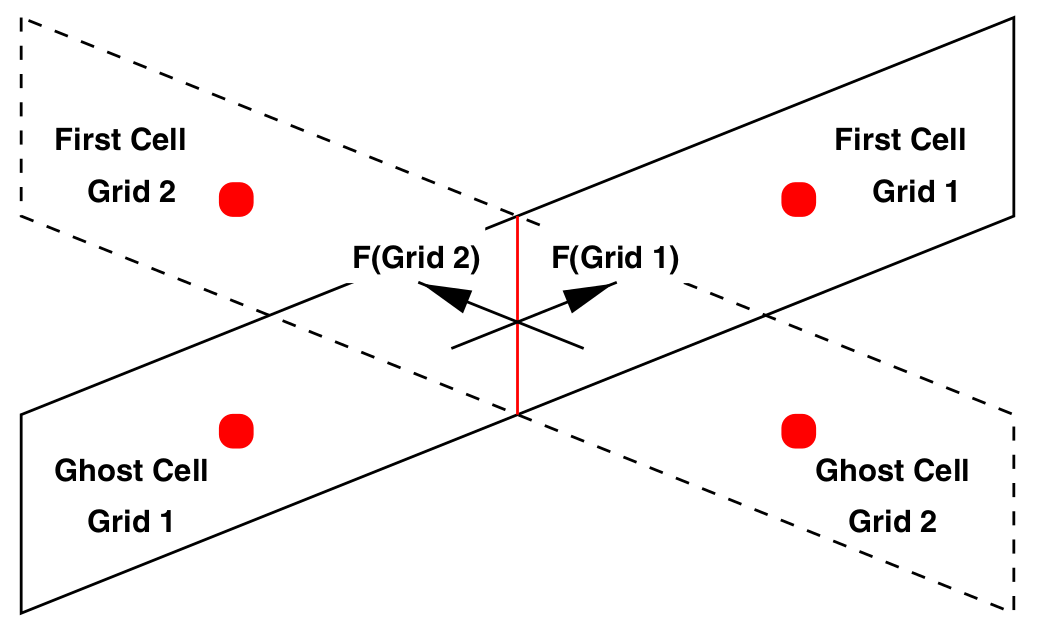
\includegraphics[width=0.5\linewidth]{flux_interface}
	\caption{Figure that illustrates the flux being computed twice on
		the cube edge, breaking the total mass conservation.
		Figure taken from \citet{ross:2006}.\label{chp5-fluxcube}}
\end{figure}

One common alternative used in the literature to handle the issue of values being defined twice at points on the
cube edges is to simply average the values (as seen in works such as \citet{ross:2006, chen:2008}).
This approach will be explored in this chapter as one of the methods.

Another alternative approach, based on Semi-Lagrangian mass corrections
(for a review of these methods, we refer to \citet{diamantakis:2014}),
involves computing the orthogonal projection of the grid function $\mathbb{D}^n$ onto the following space:
\begin{equation*}
	V_0 = \{ \delta \in \mathcal{CS}_N: \quad
		\sum_{p=1}^6 \sum_{i,j=1}^N \mathbb{\delta}_{ijp} \sigma_{ijp} \Delta x \Delta y = 0\},
\end{equation*}
where $V_0$ represents the space of functions with a zero average.
The element of $V_0$ that minimizes its distance to $\mathbb{D}^n$ in the norm 2 is given by:
\begin{equation*}
\mathbb{D}^{cor,n}_{ijp} = \mathbb{D}^n_{ijp} - \bigg(\frac{	\sum_{p=1}^6 \sum_{r,s=1}^N \mathbb{D}_{rsp}^n \sigma_{rsp} \Delta x \Delta y}
 {\sum_{p=1}^6 \sum_{r,s=1}^N \sigma_{rsp}^2 \Delta x \Delta y}\bigg)\sigma_{ijp}.
\end{equation*}
\subsection{Dimension splitting}
\label{sec-csdsplit}
In this section, we will utilize the operator splitting method described in Section \ref{sec-dsplit} 
to obtain a CS-FV scheme.
We will focus on 1D fluxes, specifically the PPM fluxes introduced in Section \ref{chp2-sec-flux},
denoted as ${F}_{i+\frac{1}{2},j,p}^n$ and ${G}_{i,j+\frac{1}{2},p}^n$.
To facilitate the scheme, we introduce the auxiliary grid functions $\mathbf{F}$ and $\mathbf{G}$ belonging to $\mathcal{CS}_{N}$, defined as follows:
\begin{align*}
	\mathbf{F}_{ijp}({Q^n,\tilde{u}^n}) = -{\lambda} \bigg({F}_{i+\frac{1}{2},j,p}^n(Q^n_{\times,j,p},\tilde{u}^n_{i+\frac{1}{2},j,p})-
	{F}_{i-\frac{1}{2},j,p}^n(Q^n_{\times,j,p},\tilde{u}^n_{i-\frac{1}{2},j,p}) \bigg),
\end{align*}
for $i=1, \ldots, N$, $j=-\nu+1, \ldots, M + \nu$, and
\begin{align*}
	\mathbf{G}_{ijp}({Q^n,\tilde{v}^n}) = -{\lambda} \bigg({G}_{i,j+\frac{1}{2},p}^n(Q^n_{i,\times,p},\tilde{v}^n_{i,j+\frac{1}{2},p})-
	{G}_{i,j-\frac{1}{2},p}^n(Q^n_{i,\times,p},\tilde{v}^n_{i,j-\frac{1}{2},p}) \bigg),
\end{align*}
for $i=-\nu+1, \ldots, N + \nu$  $j=1, \ldots, M$.
The terms $\tilde{u}^n_{i+\frac{1}{2},j,p}$ and $\tilde{v}^n_{i,j+\frac{1}{2},p}$ represent the 
time-averaged winds used in the computation of departure points in the $x$ and $y$ directions, respectively. 
These averages are calculated using either RK1 or RK2 from Section \ref{chp2-sec-dp}. 
To facilitate the description of the 1D fluxes ${F}_{i+\frac{1}{2},j,p}^n$ and ${G}_{i,j+\frac{1}{2},p}^n$, 
we introduce the time-averaged CFL numbers defined as follows:
\begin{align*}
	\tilde{c}_{i+\frac{1}{2},j,p}^{x,n} = \tilde{u}_{i+\frac{1}{2},j,p}^{x,n}\frac{\Delta t}{\Delta x},\
	\tilde{c}_{i,j+\frac{1}{2},p}^{y,n} = \tilde{v}_{i,j+\frac{1}{2},p}^{y,n}\frac{\Delta t}{\Delta y}.
\end{align*}
The discrete divergence is then obtained as:
\begin{equation}
	\mathbb{D}^n_{ijp} = -\frac{1}{\Delta t \sigma_{ijp}}
	\bigg[
	\mathbf{F}_{ijp}\bigg(Q^n + \frac{1}{2}\mathbf{g}(Q^n,\tilde{v}^n), \tilde{u}^n \bigg) 
	+\mathbf{G}_{ijp}\bigg(Q^n + \frac{1}{2}\mathbf{f}(Q^n,\tilde{u}^n), \tilde{v}^n \bigg) \bigg],
\end{equation}
where the inner advective operators $\mathbf{f}$ and $\mathbf{g}$ are given in Table \ref{chp3-tab1}.

Now, our objective is to describe the 1D fluxes ${F}_{i+\frac{1}{2},j,p}^n$ and ${G}_{i,j+\frac{1}{2},p}^n$. 
It is important to note that these fluxes depend on the edge treatment, as well as the computation of stencils, as we will see in the following sections.

\subsubsection{ET-ZA22}
We have a piecewise-parabolic approximation in the $x$ direction:
\begin{align}
	\label{chp5-ppmx-eq1}
	\begin{cases}
		q_{ij}^x(x;Q_{\times, j}^n) = q_{L,i,j}^x + \Delta q_{ij}^x z_i(x) + q_{6, i,j}^xz_i(x)(1-z_i(x)), \\
		z_i(x) = \frac{x-x_{i-\frac{1}{2}}}{\Delta x},
		\quad x \in X_i,\\
		q_{L, i,j}^x = q_{i-\frac{i}{2},j}^n+ O(\Delta x^2),\\
		q_{R, i,j}^x = q_{i+\frac{i}{2},j}^n+ O(\Delta x^2),\\
		\Delta q_{ij}^x = q_{R, i,j}^x - q_{L, i,j}^x,\\
		q_{6,i,j}^x = 6\bigg(Q_{ij}^n - \frac{(q_{L,i,j}^x + q_{R,i,j}^x)}{2}\bigg),
	\end{cases}
\end{align}
for $i=1, \ldots, N$, $j=-\nu+1, \ldots, M + \nu$, and we also construct a piecewise-parabolic
approximation in the $y$ direction:
\begin{align}
	\label{chp5-ppmy-eq2}
	\begin{cases}
		q_{ij}^y(y;Q_{i,\times}^n) = q_{L,i,j}^y + \Delta q_{ij}^y z_j(y) + q_{6, i,j}^yz_j(y)(1-z_j(y)),\\ 
		z_j(y) = \frac{y-y_{j-\frac{1}{2}}}{\Delta y},
		\quad y \in Y_j,\\
		q_{L, i,j}^y = q_{i,j-\frac{1}{2}}^n+ O(\Delta y^2),\\
		q_{R, i,j}^y = q_{i,j+\frac{1}{2}}^n+ O(\Delta y^2),\\
		\Delta q_{ij}^y = q_{R, i,j}^y - q_{L, i,j}^y,\\
		q_{6,i,j}^y = 6\bigg(Q_{ij}^n - \frac{(q_{L,i,j}^y + q_{R,i,j}^y)}{2}\bigg),
	\end{cases}
\end{align}
for $i=-\nu+1, \ldots, N + \nu$, $j=1, \ldots, M$.
The values $q_{L,i,j}^x$, $q_{R,i,j}^x$, $q_{L,i,j}^y$, and $q_{R,i,j}^y$,
which approximate the values of $q$ at C-grid wind positions, are computed
using one of the schemes PPM-0, PPM-PL07, PPM-CW84, or PPM-L04, as described
in Sections \ref{chp2-sec-ppm} and \ref{chp2-sec-mono}.
These approximations are expected to be
second-order accurate because the given average values are computed on the
2D control volume $\Omega_{ij}$ instead of the 1D control volumes $X_i$ or $Y_j$.
Then, we may express the fluxes as in Equation \eqref{chp-sec-flux:numerical-flux3}, namely:
\begin{align}
	\label{chp5-flux-xdir}
	F_{i+\frac{1}{2},j}^n ({Q^n_{\times,j},\tilde{u}^n_{i+\frac{1}{2},j}})= \tilde{u}^{n}_{i+\frac{1}{2},j}\times
	\begin{cases}
		q_{R,i,j}^x +\frac{1}{2}(q_{6,i,j}^x - \Delta q_{ij}^x){\tilde{c}_{i+\frac{1}{2},j}^{x,n}}
		+\frac{1}{3}{q_{6,i,j}^x}(\tilde{c}_{i+\frac{1}{2},j}^{x,n})^2,
		\quad &\text{if} \quad \tilde{u}_{i+\frac{1}{2},j}^n>0,\\
		q_{L,i+1,j}^x - \frac{1}{2}(q_{6,i+1,j}^x + \Delta q_{i+1,j}^x){\tilde{c}_{i+\frac{1}{2},j}^{x,n}}
		-\frac{1}{3}{q_{6,i+1,j}^x}(\tilde{c}_{i+\frac{1}{2},j}^{x,n})^2,
		\quad &\text{if} \quad \tilde{u}_{i+\frac{1}{2},j}^n\leq0,\\
	\end{cases}
\end{align}
for $i=0, \ldots, N$, $j=-\nu+1, \ldots, M + \nu$, and 
\begin{align}
	\label{chp5-flux-ydir}
	G_{i,j+\frac{1}{2}}^n ({Q^n_{i,\times},\tilde{v}^n_{i,j+\frac{1}{2}}})= \tilde{v}^{n}_{i,j+\frac{1}{2}}\times
	\begin{cases}
		q_{R,i,j}^y +\frac{1}{2}(q_{6,i,j}^y - \Delta q_{ij}^y){\tilde{c}_{i,j+\frac{1}{2}}^{y,n}}
		+\frac{1}{3}{q_{6,i,j}^y}(\tilde{c}_{i,j+\frac{1}{2}}^{y,n})^2,
		\quad &\text{if} \quad \tilde{v}_{i+\frac{1}{2},j}^n>0,\\
		q_{L,i,j+1}^y - \frac{1}{2}(q_{6,i,j+1}^y + \Delta q_{i,j+1}^y){\tilde{c}_{i,j+\frac{1}{2}}^{y,n}}
		-\frac{1}{3}{q_{6,i,j+1}^y}(\tilde{c}_{i,j+\frac{1}{2}}^{y,n})^2,
		\quad &\text{if} \quad \tilde{v}_{i,j+\frac{1}{2}}^n\leq0,\\
	\end{cases}
\end{align}
for $i=-\nu+1, \ldots, N + \nu$, $j=0, \ldots, M$.
\subsubsection{ET-PL07}
We have a piecewise-parabolic approximation in the $x$ direction:
\begin{align}
	\label{chp5-ppmx-eq1-pl07}
	\begin{cases}
		q_{ij}^x(x;Q_{\times, j}^n) = q_{L,i,j}^x + \Delta q_{ij}^x z_i(x) + q_{6, i,j}^xz_i(x)(1-z_i(x)), \\
		z_i(x) = \frac{x-x_{i-\frac{1}{2}}}{\Delta x},
		\quad x \in X_i,\\
		q_{L, i,j}^x = q_{i-\frac{i}{2},j}^n+ O(\Delta x^2),\\
		q_{R, i,j}^x = q_{i+\frac{i}{2},j}^n+ O(\Delta x^2),\\
		\Delta q_{ij}^x = q_{R, i,j}^x - q_{L, i,j}^x,\\
		q_{6,i,j}^x = 6\bigg(Q_{ij}^n - \frac{(q_{L,i,j}^x + q_{R,i,j}^x)}{2}\bigg),
	\end{cases}
\end{align}
for $i=1, \ldots, N$, $j=-\nu+1, \ldots, M + \nu$, and we also construct a piecewise-parabolic
approximation in the $y$ direction:
\begin{align}
	\label{chp5-ppmy-pl07}
	\begin{cases}
		q_{ij}^y(y;Q_{i,\times}^n) = q_{L,i,j}^y + \Delta q_{ij}^y z_j(y) + q_{6, i,j}^yz_j(y)(1-z_j(y)),\\ 
		z_j(y) = \frac{y-y_{j-\frac{1}{2}}}{\Delta y},
		\quad y \in Y_j,\\
		q_{L, i,j}^y = q_{i,j-\frac{1}{2}}^n+ O(\Delta y^2),\\
		q_{R, i,j}^y = q_{i,j+\frac{1}{2}}^n+ O(\Delta y^2),\\
		\Delta q_{ij}^y = q_{R, i,j}^y - q_{L, i,j}^y,\\
		q_{6,i,j}^y = 6\bigg(Q_{ij}^n - \frac{(q_{L,i,j}^y + q_{R,i,j}^y)}{2}\bigg),
	\end{cases}
\end{align}
for $i=-\nu+1, \ldots, N + \nu$, $j=1, \ldots, M$.
The values $q_{L,i,j}^x$, $q_{R,i,j}^x$, $q_{L,i,j}^y$, and $q_{R,i,j}^y$,
which approximate the values of $q$ at C-grid wind positions, are computed
using one of the schemes PPM-0, PPM-PL07, PPM-CW84, or PPM-L04, as described
in Sections \ref{chp2-sec-ppm} and \ref{chp2-sec-mono}.
These approximations are expected to be
second-order accurate because the given average values are computed on the
2D control volume $\Omega_{ij}$ instead of the 1D control volumes $X_i$ or $Y_j$.
Then, we may express the fluxes as in Equation \eqref{chp-sec-flux:numerical-flux3}, namely:
\begin{align}
	\label{chp5-flux-xdir--pl07}
	F_{i+\frac{1}{2},j}^n ({Q^n_{\times,j},\tilde{u}^n_{i+\frac{1}{2},j}})= \tilde{u}^{n}_{i+\frac{1}{2},j}\times
	\begin{cases}
		q_{R,i,j}^x +\frac{1}{2}(q_{6,i,j}^x - \Delta q_{ij}^x){\tilde{c}_{i+\frac{1}{2},j}^{x,n}}
		+\frac{1}{3}{q_{6,i,j}^x}(\tilde{c}_{i+\frac{1}{2},j}^{x,n})^2,
		\quad &\text{if} \quad \tilde{u}_{i+\frac{1}{2},j}^n>0,\\
		q_{L,i+1,j}^x - \frac{1}{2}(q_{6,i+1,j}^x + \Delta q_{i+1,j}^x){\tilde{c}_{i+\frac{1}{2},j}^{x,n}}
		-\frac{1}{3}{q_{6,i+1,j}^x}(\tilde{c}_{i+\frac{1}{2},j}^{x,n})^2,
		\quad &\text{if} \quad \tilde{u}_{i+\frac{1}{2},j}^n\leq0,\\
	\end{cases}
\end{align}
for $i=0, \ldots, N$, $j=-\nu+1, \ldots, M + \nu$, and 
\begin{align}
	\label{chp5-flux-ydir-pl07}
	G_{i,j+\frac{1}{2}}^n ({Q^n_{i,\times},\tilde{v}^n_{i,j+\frac{1}{2}}})= \tilde{v}^{n}_{i,j+\frac{1}{2}}\times
	\begin{cases}
		q_{R,i,j}^y +\frac{1}{2}(q_{6,i,j}^y - \Delta q_{ij}^y){\tilde{c}_{i,j+\frac{1}{2}}^{y,n}}
		+\frac{1}{3}{q_{6,i,j}^y}(\tilde{c}_{i,j+\frac{1}{2}}^{y,n})^2,
		\quad &\text{if} \quad \tilde{v}_{i+\frac{1}{2},j}^n>0,\\
		q_{L,i,j+1}^y - \frac{1}{2}(q_{6,i,j+1}^y + \Delta q_{i,j+1}^y){\tilde{c}_{i,j+\frac{1}{2}}^{y,n}}
		-\frac{1}{3}{q_{6,i,j+1}^y}(\tilde{c}_{i,j+\frac{1}{2}}^{y,n})^2,
		\quad &\text{if} \quad \tilde{v}_{i,j+\frac{1}{2}}^n\leq0,\\
	\end{cases}
\end{align}
for $i=-\nu+1, \ldots, N + \nu$, $j=0, \ldots, M$.

\section{Numerical experiments}
\label{chp-cs-numexpadv}


\section{Concluding remarks}
\label{chp-cs-conc}